% S7 project report: DDoS Mitigation using AI in SDN
% Build:  pdflatex s7_report.tex   (run it twice so the contents page fills in)
% Figures are in the figures/ folder next to this file.
\documentclass[12pt,a4paper]{article}

\usepackage[margin=1in]{geometry}
\usepackage{graphicx}
\usepackage{amsmath}
\usepackage{booktabs}
\usepackage{float}
\usepackage{parskip}
\usepackage{listings}
\usepackage{fancyhdr}
\usepackage{tikz}
\usetikzlibrary{positioning,arrows.meta,fit,backgrounds,calc}
\usepackage[hidelinks]{hyperref}

\graphicspath{{figures/}}
\renewcommand{\labelitemi}{$\bullet$}
\renewcommand{\labelitemiii}{$\ast$}
\renewcommand{\labelitemiv}{$\cdot$}

% ---- change these two lines when you submit ----
\newcommand{\reportdate}{26 November 2026}
\newcommand{\reportmonth}{November 2026}

\setlength{\headheight}{14.5pt}
\pagestyle{fancy}
\fancyhf{}
\lhead{\reportmonth}
\rhead{SDN DDoS}
\cfoot{\thepage}

\lstset{
  language=Python,
  basicstyle=\ttfamily\small,
  keywordstyle=\bfseries,
  columns=fullflexible,
  showstringspaces=false,
  captionpos=t,
  xleftmargin=1em,
}

\begin{document}

% =====================================================================
% Title page
% =====================================================================
\begin{titlepage}
\centering
\vspace*{2cm}
{\LARGE\bfseries DDoS Mitigation using AI in SDN\par}
\vspace{3cm}
{\large\itshape Submitted by:\par}
\vspace{0.4cm}
{\large\bfseries Anirudh Nambiar B230629CS\par}
\vspace{0.3cm}
{\large\itshape Project Guide:\par}
\vspace{0.4cm}
{\large\bfseries Dr Arun Raj Kumar P\par}
\vspace{0.1cm}
Associate Professor, CSED\par
\vspace{2.5cm}

\includegraphics[width=3.5cm]{nitc_logo.png}\par
\vfill
Department of Computer Science \& Engineering\par
\textbf{National Institute of Technology Calicut}\par
\reportdate\par
\end{titlepage}

% =====================================================================
% Abstract
% =====================================================================
\begin{abstract}
The project addresses the problem of security vulnerabilities within
Software-Defined Networking (SDN), specifically focusing on the detection and
mitigation of Distributed Denial of Service (DDoS) attacks targeting the SDN
infrastructure and network availability. Recent SDN security research focuses on
dynamic detection techniques rather than fixed threshold methods. The literature
highlights future research directions that need to be looked into by the
community such as Coordinated spoofed three-way handshake attack in SDN,
Combined DHCP exhaustion and slow-rate TCAM DDoS attack in SDN, LDoS Attacks and
many more. Several approaches have been proposed, including statistical traffic
analysis, information-theoretic measures like Generalized Entropy, and various
supervised Machine Learning classifiers, which have shown promising results under
certain conditions. However, the literature reveals several open problems such as
high false-positive rates during flash-crowd events, the trade-off between
detection speed and accuracy for low-rate (LDoS) attacks, and the resource
bottlenecks created by centralized decision-making in the SDN control plane.
These limitations reduce the effectiveness of current SDN defense systems in
practical deployments. The primary objectives of this project are to develop a
lightweight, intelligent detection framework capable of distinguishing stealthy
Low-Rate DDoS (LDoS) attacks from legitimate flash crowds, and to implement an
adaptive mitigation strategy that minimizes computational overhead on the SDN
controller. To achieve these objectives, the project plans to follow a structured
methodology that includes a comprehensive literature survey, realistic network
topology generation using Mininet, testing using a diverse dataset containing
both flooding and LDoS traffic scenarios, development of the detection model
using advanced machine learning techniques, and rigorous performance evaluation
against standard metrics. The proposed system is intended to improve attack
detection while keeping controller overhead low as well as Quality of Service
(QoS) even under complex, multi-vector attack conditions.

\vspace{1em}
\noindent\textbf{Keywords:} Software-Defined Networking (SDN), DDoS Mitigation,
Network Security
\end{abstract}

\newpage
\tableofcontents

% =====================================================================
\newpage
\section{Introduction}
% =====================================================================
Software Defined Networking (SDN) is a modern networking architecture that
separates the control plane (decision-making) from the data plane (packet
forwarding). This separation enables centralized and programmable network
management. SDN is widely used in data centers, cloud infrastructures, enterprise
WANs, and telecommunication backbone networks.

Traditional networks are generally hardware-dependent and difficult to manage
dynamically. SDN improves flexibility by allowing network administrators to
configure and manage the network through software. It also enables faster
response to traffic changes and simplifies network management.

An SDN architecture mainly consists of the following three layers:
\begin{itemize}
  \item \textbf{Application Layer}\\
  This layer contains network applications and services such as firewalls, load
  balancers, and traffic monitoring systems. These applications communicate
  network policies to the controller using the Northbound Interface.
  \item \textbf{Control Layer}\\
  The control layer contains the logically centralized SDN controller, which acts
  as the network operating system. It manages flow rules, network topology, and
  communicates with switches through the Southbound Interface.
  \item \textbf{Data Layer}\\
  This layer consists of programmable forwarding devices such as switches and
  routers. These devices forward packets based on flow rules installed by the
  controller. The rules are generally stored in TCAM/CAM memory for fast lookup
  operations.
\end{itemize}

\begin{figure}[H]
  \centering
  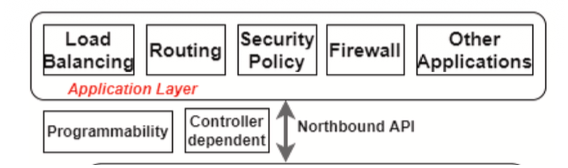
\includegraphics[width=0.85\linewidth]{application_layer.png}
  \caption{Application Layer in SDN Architecture (Adapted from \cite{sinha2025})}
\end{figure}

\begin{figure}[H]
  \centering
  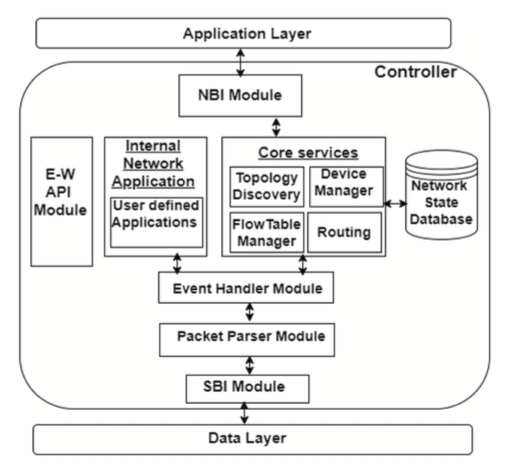
\includegraphics[width=0.6\linewidth]{control_layer.png}
  \caption{Control Layer and SDN Controller (Adapted from \cite{sinha2025})}
\end{figure}

\begin{figure}[H]
  \centering
  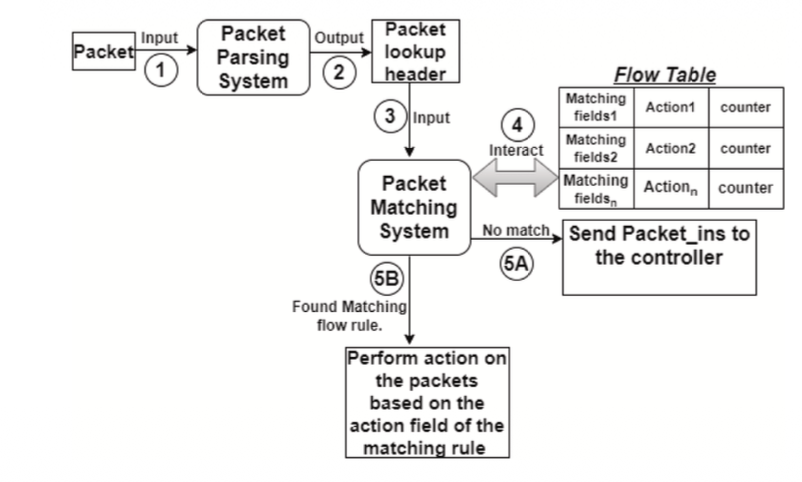
\includegraphics[width=0.75\linewidth]{data_layer.png}
  \caption{Data Layer and Packet Forwarding (Adapted from \cite{sinha2025})}
\end{figure}

% =====================================================================
\newpage
\section{OpenFlow Protocol}
% =====================================================================
OpenFlow is the most widely adopted Southbound Interface protocol in SDN. It is
how the controller communicates with the data plane, i.e.\ the switches.
\begin{itemize}
  \item Establishes a secure communication channel (TLS/TCP) between the
  controller and each switch.
  \item The controller maintains one OpenFlow module per switch; each switch has a
  single module.
  \item Communication is done via OpenFlow messages:
  \begin{itemize}
    \item Packet in -- switch forwards unmatched packet to controller
    \item Flow mod -- controller installs/modifies flow rules on switch
    \item Packet out -- controller instructs switch to forward a packet
  \end{itemize}
\end{itemize}

\begin{figure}[H]
  \centering
  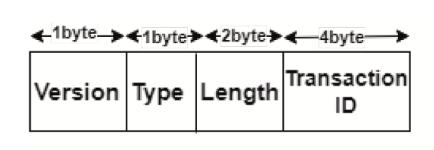
\includegraphics[width=0.75\linewidth]{openflow_header.png}
  \caption{OpenFlow Packet header}
\end{figure}

% =====================================================================
\newpage
\section{Types of DDoS Attacks}
% =====================================================================
The two main primary categories are
\begin{itemize}
  \item Capacity Attacks -- Generate massive traffic to exhaust bandwidth,
  controller resources, or network processing capacity.
  \item Low Rate Attacks -- Send stealthy traffic that mimics normal behavior,
  making them harder to detect.
  \item Flooding Attacks (Capacity Based)
  \begin{itemize}
    \item SYN Flood
    \item UDP Flood
    \item ICMP Flood
    \item HTTP Flood
  \end{itemize}
  \item Amplification Attacks
  \begin{itemize}
    \item DNS Amplification
    \item NTP Amplification
    \item SSDP Amplification
  \end{itemize}
  \item Low Rate Attacks
  \begin{itemize}
    \item Slowloris Attack
    \item Shrew Attack
  \end{itemize}
\end{itemize}

% =====================================================================
\newpage
\section{SDN Vulnerabilities}
% =====================================================================
\begin{itemize}
  \item \textbf{Single Point of Failure (SPOF)}
  \begin{itemize}
    \item The centralized SDN controller, while powerful, introduces a critical
    vulnerability as it acts as a Single Point of Failure (SPOF).
    \item If the controller becomes unavailable, the entire network loses its
    decision-making capability, and switches can only act on existing flow rules.
    \item Switches in pure SDN have no fallback routing logic, meaning new flows
    cannot be handled without the controller.
    \item This makes the controller a prime target for DDoS attacks, as taking it
    down can effectively paralyze the network.
  \end{itemize}
  \item \textbf{Distributed Controller Challenges}
  \begin{itemize}
    \item Distributed controllers partially mitigate this issue by allowing
    multiple controllers to share the control plane.
    \item However, distribution introduces synchronization overhead since
    controllers must maintain a consistent global network view.
    \item This synchronization increases latency and complexity.
    \item The East-West interface responsible for controller synchronization can
    itself become a bottleneck under high load.
  \end{itemize}
  \item \textbf{Hybrid SDN Tradeoff}
  \begin{itemize}
    \item In Hybrid SDN, legacy devices can continue operating independently,
    reducing the impact of controller failure.
    \item However, this comes at the cost of reduced programmability and
    centralized control.
  \end{itemize}
  \item \textbf{Southbound Interface Bottleneck}
  \begin{itemize}
    \item The Southbound Interface (SBI) channel between the controller and
    switches carries:
    \begin{itemize}
      \item Flow rule installation messages
      \item Statistics polling messages
      \item Packet in messages
    \end{itemize}
    \item High-rate DDoS traffic can saturate this channel, delaying legitimate
    flow rule updates.
  \end{itemize}
  \item \textbf{Security Implication}
  \begin{itemize}
    \item These bottlenecks are directly exploited by DDoS attacks.
    \item As a result, SDN can become more vulnerable than traditional networks
    if proper mitigation mechanisms are not implemented.
  \end{itemize}
\end{itemize}

% =====================================================================
\newpage
\section{Existing Solutions}
% =====================================================================
\begin{itemize}
  \item \textbf{Statistical Detection Methods}
  \begin{itemize}
    \item Statistical methods analyze flow-level traffic metrics collected from
    the SDN controller and switches to detect anomalies.
  \end{itemize}
  \item \textbf{How It Works}
  \begin{itemize}
    \item Traffic features monitored periodically include:
    \begin{itemize}
      \item Packet rate
      \item Byte count
      \item Flow count
      \item Destination IP distribution
    \end{itemize}
    \item Anomalies are detected when:
    \begin{itemize}
      \item Metrics exceed predefined thresholds
      \item Entropy values drop significantly
    \end{itemize}
  \end{itemize}
\end{itemize}

\begin{itemize}
  \item \textbf{Machine Learning Based Detection Methods}
  \begin{itemize}
    \item Standard Machine Learning (ML) approaches train classifiers on
    flow-level features extracted from the SDN controller's flow tables.
    \item The goal is to distinguish malicious traffic from legitimate network
    traffic.
  \end{itemize}
  \item \textbf{Common Algorithms}
  \begin{itemize}
    \item Decision Trees and Random Forest
    \begin{itemize}
      \item Interpretable models
      \item Fast inference speed
    \end{itemize}
    \item Support Vector Machines (SVM)
    \begin{itemize}
      \item Effective in high-dimensional feature spaces
    \end{itemize}
    \item K-Nearest Neighbors (KNN)
    \begin{itemize}
      \item Instance-based learning approach
      \item Does not require a separate training phase
    \end{itemize}
    \item Deep Learning Based Detection Methods
    \begin{itemize}
      \item Deep Learning approaches automatically learn hierarchical traffic
      representations from raw or minimally processed flow data.
      \item This reduces the need for manual feature engineering.
    \end{itemize}
    \item Common Architectures
    \begin{itemize}
      \item Convolutional Neural Networks (CNN)
      \begin{itemize}
        \item Capture spatial patterns in traffic feature matrices.
      \end{itemize}
      \item Recurrent Neural Networks (RNN) / Long Short-Term Memory (LSTM)
      \begin{itemize}
        \item Model sequential and temporal dependencies in network traffic
        flows.
      \end{itemize}
      \item Autoencoders
      \begin{itemize}
        \item Used for unsupervised anomaly detection.
        \item Learn to reconstruct normal traffic behavior.
        \item High reconstruction error indicates possible attack traffic.
      \end{itemize}
    \end{itemize}
  \end{itemize}
\end{itemize}

% =====================================================================
\newpage
\section{Limitations of Existing Solutions}
% =====================================================================
\begin{itemize}
  \item \textbf{Limitations of Statistical Methods}
  \begin{itemize}
    \item Unable to effectively detect:
    \begin{itemize}
      \item Low-rate attacks
      \item Slow-rate attacks
    \end{itemize}
    since traffic volumes may still appear normal.
    \item Cannot reliably distinguish between:
    \begin{itemize}
      \item Flash crowds and DDoS attacks
    \end{itemize}
    because both can produce similar entropy drops.
    \item Mitigation strategies may block all traffic directed to the victim,
    resulting in legitimate service downtime.
    \item Static thresholds are not adaptive and fail to adjust to changing
    baseline traffic patterns.
  \end{itemize}
\end{itemize}

\begin{itemize}
  \item \textbf{Limitations of Machine Learning Methods}
  \begin{itemize}
    \item Requires large labelled training datasets, which are difficult to
    obtain for SDN-specific environments.
    \item Extensive feature extraction increases the computational burden on the
    controller, which is already a bottleneck in real deployments.
    \item Models become static after training and are unable to adapt to:
    \begin{itemize}
      \item New attack patterns
      \item Evolving attack strategies
    \end{itemize}
    without retraining.
    \item Performance degrades significantly when evaluated on traffic
    distributions that differ from the training dataset.
  \end{itemize}
\end{itemize}

\begin{itemize}
  \item \textbf{Limitations of Deep Learning Methods}
  \begin{itemize}
    \item High computational cost:
    \begin{itemize}
      \item Inference latency may be too high for real-time SDN deployments.
    \end{itemize}
    \item Requires large amounts of training data:
    \begin{itemize}
      \item SDN-specific labelled datasets are limited and difficult to obtain.
    \end{itemize}
  \end{itemize}
\end{itemize}

% =====================================================================
\newpage
\section{Proposed System Design}
% =====================================================================
The limitations above point to a basic dilemma. A detector with a fixed
baseline (a static threshold) raises false alarms whenever real traffic grows,
for example during a flash crowd. A detector that keeps re-learning its
baseline (an adaptive or online-learning detector) accepts real growth, but it
can also be taught to accept an attack. If an attacker raises the flood
\emph{slowly}, every step looks normal, the detector learns it, and the flood
can reach many times the normal rate without a single alarm. This is called a
\textbf{frog-boiling attack}. It is known from other areas of anomaly detection
\cite{antidote,chantin}, but it has not been studied for SDN DDoS detectors.
A recent Mininet/Ryu detector with an adaptive threshold \cite{zhang2026}
explicitly leaves such attackers out of scope.

The proposed system is called \textbf{Evidence-Gated Learning (EGL)}. Its main
idea is simple: \emph{a detector may only learn from traffic that the network
can vouch for}. Every web visit is a TCP connection. The client opens it with a
SYN and the server closes it with a FIN. Real users finish their connections,
even when a sudden crowd arrives. Spoofed SYNs from an attacker never do. The
controller therefore measures a \textbf{completion ratio},
\begin{equation}
  e_n = \frac{\text{FINs sent by the server}}{\text{SYNs sent to the server}}
  \quad\text{(over the last 5 seconds)},
\end{equation}
which stays close to 1 for real users and drops to about $1/m$ when the attack
is $m$ times the users' rate. A \textbf{Learning Gate} lets the detector update
its idea of ``normal'' only while $e_n \ge \tau$ (we use $\tau = 0.7$). The gate
never raises alarms itself; it only decides what the detector is allowed to
learn. The idea of comparing SYNs and FINs comes from early SYN flood detection
\cite{wang2002}; here it is used to protect a learning detector.

The architecture is designed to handle the following types of attacks:
\begin{itemize}
  \item High-volume flooding attacks (abrupt TCP SYN floods)
  \item Slow-ramp (frog-boiling) SYN floods that try to be learned as normal
  \item Distributed attacks sent from several hosts on different switches
\end{itemize}

The system consists of four functional components that operate together within
the Ryu controller, as shown in Figure~\ref{fig:design}:
\begin{itemize}
  \item \textbf{Telemetry:} Flow rules on the switch count the SYNs sent to the
  server and the FINs sent back by the server, by matching on TCP flags. The
  controller reads these counters once per second. No packets are sent to the
  controller for this, so the load on the controller does not grow with the
  attack.
  \item \textbf{Detector:} A lightweight detector watches the SYN rate and
  raises an alarm when it is unusually high. Three detectors are compared:
  a static z-score threshold, an EWMA (exponentially weighted moving average)
  detector, and Half-Space Trees \cite{tan2011}, an online machine learning
  anomaly detector.
  \item \textbf{Learning Gate:} Allows the detector to learn only while the
  completion ratio is at least $\tau$. It also keeps a \emph{trusted baseline}:
  the median SYN rate of the seconds it approved.
  \item \textbf{Mitigator:} When an alarm is raised, it rate-limits new
  connections from unknown sources with an OpenFlow meter, while clients that
  have already completed a connection (\emph{verified clients}) get a rule that
  skips the meter.
\end{itemize}

The completion evidence cannot be faked by an attacker from outside. The FINs
are counted only on the switch port that the server is connected to, so packets
from any other host never match that rule. The system can be used with any
detector that learns online, because the gate only controls \emph{when} the
detector learns, not \emph{how} it detects.

Once an attack is detected, the system applies targeted mitigation. Instead of
blocking all traffic towards the server, it limits only the traffic that it
cannot verify. This ensures that legitimate users keep their service while the
spoofed flood is held back.

\begin{figure}[H]
\centering
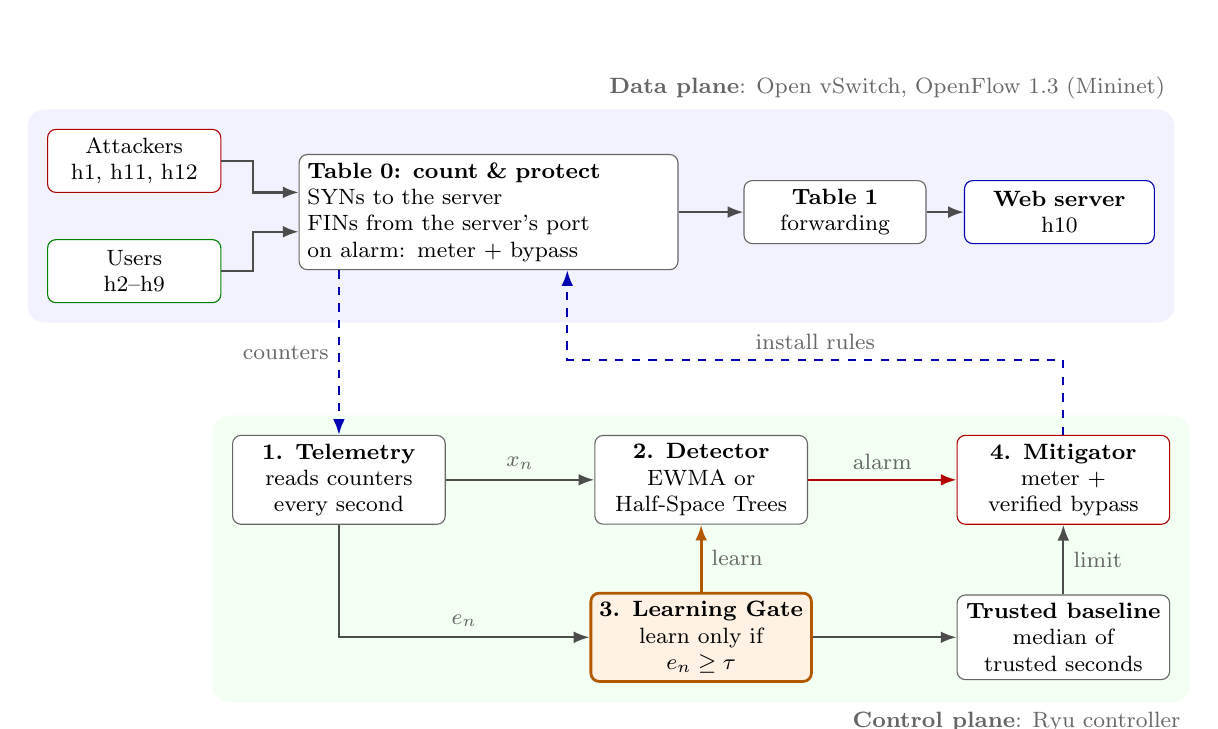
\begin{tikzpicture}[x=1cm,y=1cm,
  box/.style={draw=black!60, rounded corners=3pt, fill=white, align=center,
              font=\footnotesize, inner sep=3pt, minimum height=8mm},
  host/.style={box, minimum width=22mm},
  stage/.style={box, minimum width=27mm},
  gatebox/.style={box, line width=1pt, fill=orange!10, draw=orange!70!black, minimum width=27mm},
  arr/.style={-{Latex[length=2mm]}, black!70, thick},
  ctl/.style={-{Latex[length=2mm]}, blue!70!black, thick, dashed},
  lbl/.style={font=\footnotesize, text=black!60, align=center},
  zone/.style={rounded corners=6pt, inner sep=7pt}]
% data plane
\node[host, draw=red!70!black] (bots) at (0,0.65) {Attackers\\h1, h11, h12};
\node[host, draw=green!50!black] (users) at (0,-0.75) {Users\\h2--h9};
\node[box, align=left, text width=46mm] (t0) at (4.5,0) {\textbf{Table 0: count \& protect}\\
  SYNs to the server\\ FINs from the server's port\\ on alarm: meter + bypass};
\node[box, text width=21mm] (t1) at (8.9,0) {\textbf{Table 1}\\forwarding};
\node[box, text width=22mm, draw=blue!70!black] (srv) at (11.75,0) {\textbf{Web server}\\h10};
\draw[arr] (bots.east) -- ++(0.4,0) |- ($(t0.west)+(0,0.25)$);
\draw[arr] (users.east) -- ++(0.4,0) |- ($(t0.west)+(0,-0.25)$);
\draw[arr] (t0) -- (t1);
\draw[arr] (t1) -- (srv);
\begin{scope}[on background layer]
  \node[zone, fill=blue!5, fit=(bots)(users)(t0)(t1)(srv)] (dp) {};
\end{scope}
\node[lbl, anchor=south east] at (dp.north east) {\textbf{Data plane}: Open vSwitch, OpenFlow 1.3 (Mininet)};
% control plane
\node[stage] (poll) at (2.6,-3.4) {\textbf{1. Telemetry}\\reads counters\\every second};
\node[stage] (det)  at (7.2,-3.4) {\textbf{2. Detector}\\EWMA or\\Half-Space Trees};
\node[stage, draw=red!70!black] (mit) at (11.8,-3.4) {\textbf{4. Mitigator}\\meter +\\verified bypass};
\node[gatebox] (gate) at (7.2,-5.4) {\textbf{3. Learning Gate}\\learn only if\\$e_n \ge \tau$};
\node[stage] (anchor) at (11.8,-5.4) {\textbf{Trusted baseline}\\median of\\trusted seconds};
\draw[arr] (poll) -- node[lbl, above]{$x_n$} (det);
\draw[arr, red!70!black] (det) -- node[lbl, above]{alarm} (mit);
\draw[arr] (poll.south) |- node[lbl, above, pos=0.75]{$e_n$} (gate.west);
\draw[arr, orange!70!black, line width=1pt] (gate) -- node[lbl, right]{learn} (det);
\draw[arr] (gate) -- (anchor);
\draw[arr] (anchor) -- node[lbl, right]{limit} (mit);
\begin{scope}[on background layer]
  \node[zone, fill=green!5, fit=(poll)(det)(mit)(gate)(anchor)] (cp) {};
\end{scope}
\node[lbl, anchor=north east] at (cp.south east) {\textbf{Control plane}: Ryu controller};
% control channel
\draw[ctl] (t0.south -| poll) -- node[lbl, left]{counters} (poll.north);
\draw[ctl] (mit.north) -- ++(0,0.95) -| node[lbl, above, pos=0.25]{install rules} ($(t0.south)+(1.0,0)$);
\end{tikzpicture}
\caption{High Level System Design}
\label{fig:design}
\end{figure}

This design attempts to balance detection accuracy with controller performance.
The detector stays lightweight and adaptive, the gate stops it from being
poisoned by slow attacks, and the mitigation keeps real users connected, while
the controller only reads a few counters every second.

% =====================================================================
\newpage
\section{Implementation and Experimental Setup}
% =====================================================================
The system was implemented in Python as three Ryu applications
(\texttt{egl\_controller}, \texttt{detector\_app} and \texttt{mitigator\_app})
running on Ryu 4.34 with OpenFlow 1.3. The network is emulated in Mininet with
Open vSwitch. All the code, results and figures are in the project repository
(\texttt{github.com/Anirudh-N-15/mininet}, branch \texttt{egl}). The work was
carried out step by step, and each step has its own run script and check.

\subsection{Network Topology Setup}
The experiments use one three-switch topology with twelve hosts. Two access
switches (s1 and s2) are connected to a central switch (s3). Hosts h1--h5 and
h11 are connected to s1, hosts h6--h10 to s2, and h12 to s3
(Figure~\ref{fig:topo}).

The roles of the hosts are:
\begin{itemize}
  \item \textbf{h10 (10.0.0.10)} is the protected web server, on port 6 of s2.
  \item \textbf{h1, h11 and h12} are the attackers. They are placed on all three
  switches, so the attack is a real distributed attack.
  \item \textbf{h2, h3, h4, h6, h7, h8, h9} run the legitimate users.
  \item \textbf{h5} acts as the default gateway of the server, so the server's
  replies to spoofed addresses leave the network as they would in a real
  deployment.
\end{itemize}

\begin{lstlisting}[caption={Mininet Topology for the Experiments}]
from mininet.topo import Topo

class EGLTopology(Topo):
    def build(self, datapath="kernel"):
        opts = dict(protocols="OpenFlow13", datapath=datapath)
        s1 = self.addSwitch("s1", dpid="1", **opts)
        s2 = self.addSwitch("s2", dpid="2", **opts)
        s3 = self.addSwitch("s3", dpid="3", **opts)
        self.addLink(s1, s3)
        self.addLink(s2, s3)
        for n in range(1, 6):
            self.addLink(self.addHost("h%d" % n,
                         ip="10.0.0.%d/24" % n), s1)
        for n in range(6, 11):
            self.addLink(self.addHost("h%d" % n,
                         ip="10.0.0.%d/24" % n), s2)
        # extra attackers on two other switches
        self.addLink(self.addHost("h11", ip="10.0.0.11/24"), s1)
        self.addLink(self.addHost("h12", ip="10.0.0.12/24"), s3)
\end{lstlisting}

\begin{figure}[H]
\centering
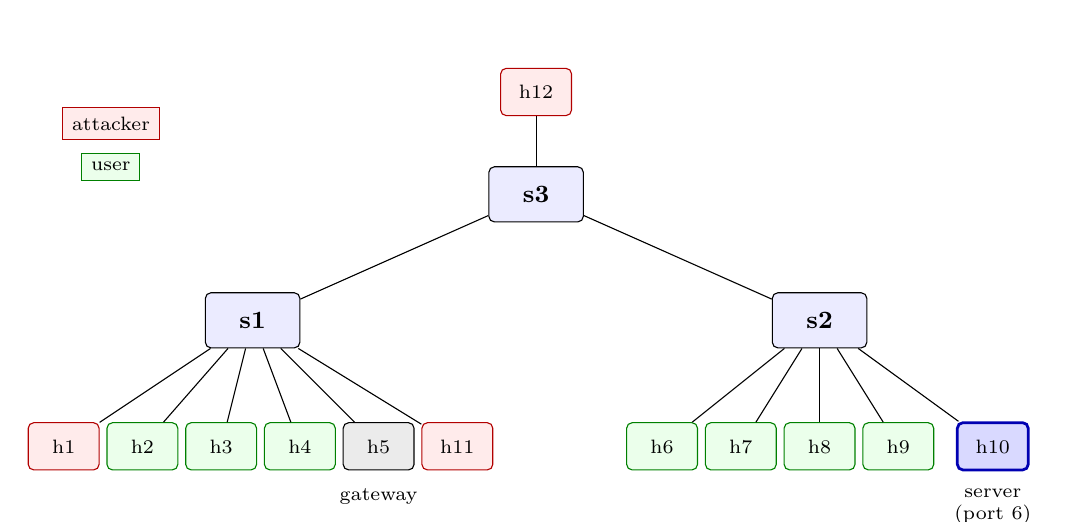
\begin{tikzpicture}[
  sw/.style={draw, rounded corners=2pt, fill=blue!8, minimum width=12mm, minimum height=7mm, font=\small\bfseries},
  hs/.style={draw, rounded corners=2pt, minimum width=9mm, minimum height=6mm, font=\scriptsize, align=center},
  atk/.style={hs, draw=red!70!black, fill=red!8},
  usr/.style={hs, draw=green!50!black, fill=green!8},
  srv/.style={hs, draw=blue!70!black, fill=blue!15, line width=1pt},
  gw/.style={hs, fill=black!8}]
\node[sw] (s3) at (0,0) {s3};
\node[sw] (s1) at (-3.6,-1.6) {s1};
\node[sw] (s2) at (3.6,-1.6) {s2};
\node[atk] (h12) at (0,1.3) {h12};
\draw (s3) -- (h12);
\draw (s1) -- (s3) -- (s2);
\foreach \n/\x/\st in {h1/-6.0/atk, h2/-5.0/usr, h3/-4.0/usr, h4/-3.0/usr, h5/-2.0/gw, h11/-1.0/atk}{
  \node[\st] (\n) at (\x,-3.2) {\n}; \draw (s1) -- (\n);}
\foreach \n/\x/\st in {h6/1.6/usr, h7/2.6/usr, h8/3.6/usr, h9/4.6/usr, h10/5.8/srv}{
  \node[\st] (\n) at (\x,-3.2) {\n}; \draw (s2) -- (\n);}
\node[font=\scriptsize, below=1mm of h10, align=center] {server\\(port 6)};
\node[font=\scriptsize, below=1mm of h5, align=center] {gateway};
\node[draw=red!70!black, fill=red!8, font=\scriptsize] at (-5.4,0.9) {attacker};
\node[draw=green!50!black, fill=green!8, font=\scriptsize] at (-5.4,0.35) {user};
\end{tikzpicture}
\caption{Mininet Topology Used for the Experiments}
\label{fig:topo}
\end{figure}

The server runs a threaded Python web server with a listen backlog of 511 (the
default of nginx and Apache) and with SYN cookies turned off, so that half-open
connections build up as they do on an unprotected server. In the mitigation
experiments every user host sends requests from a pool of 20 different
addresses, and the server treats every visitor as a first-time visitor.

\subsection{Ryu-Based Traffic Monitoring}
The monitoring component installs a two-table pipeline on the switch that the
server is connected to (s2). Table 0 counts and protects; table 1 performs
normal MAC-learning forwarding. Table 0 contains counting rules that match on
TCP flags (an ONF extension to OpenFlow 1.3, standard from OpenFlow 1.5,
supported by Open vSwitch and Ryu):
\begin{itemize}
  \item \textbf{Client SYNs to the server:} SYN flag set and ACK flag clear,
  i.e.\ a new connection attempt.
  \item \textbf{Server FINs:} FIN flag set, coming from the server and arriving
  on the server's own port (port 6). These show completed connections.
  \item \textbf{Server SYN-ACKs:} used to check that the server is answering.
\end{itemize}
Each rule counts its packets and then sends them on to table 1, so the
forwarding of the traffic is not changed.

\begin{lstlisting}[caption={Matches for the SYN and FIN Counting Rules}]
def syn_fields(cfg):
    """A client's connection attempt (SYN set, ACK clear)."""
    return dict(eth_type=IPV4, ip_proto=TCP,
                ipv4_dst=cfg.server_ip, tcp_dst=cfg.server_tcp_port,
                tcp_flags=(SYN, SYN | ACK))

def fin_fields(cfg):
    """A FIN sent by the server, on the server's own port."""
    return dict(in_port=cfg.server_ofport, eth_type=IPV4,
                ip_proto=TCP, ipv4_src=cfg.server_ip,
                tcp_src=cfg.server_tcp_port, tcp_flags=(FIN, FIN))
\end{lstlisting}

The controller requests the flow statistics of table 0 and the port statistics
of the server's port once every second. By comparing consecutive readings it
calculates the rates for each one-second window. Unlike the earlier version of
the project, the monitoring does not use Packet-In messages, so the controller's
load stays the same however large the attack is.

The main traffic features calculated by the monitoring component are:
\begin{itemize}
  \item SYN rate to the server, $x_n$
  \item FIN rate from the server
  \item SYN-ACK rate from the server
  \item Packets transmitted to the server
  \item Completion ratio $e_n$ (FINs / SYNs over the last 5 seconds; it is left
  empty when fewer than 3 SYNs were seen, as there is too little traffic)
\end{itemize}
Each window is published inside the controller as an event for the detector
application and is also stored in CSV format with its timestamp.

\subsection{Lightweight Anomaly Detection}
Three lightweight detectors were implemented behind one common interface. Each
second, a detector first \emph{scores} the window (alarm or no alarm) and then
\emph{learns} from it, but only if it did not raise an alarm and if learning is
allowed. Each detector first observes normal traffic during a warm-up period,
and it raises no alarms during that time. The detectors see only the traffic
rates, never the completion ratio, so any improvement comes from the gate alone.

\textbf{Static.} The z-score detector of the earlier version is kept as the
fixed-baseline method. It takes the mean $\mu$ and standard deviation $\sigma$
of the SYN rate during warm-up and raises an alarm when
\begin{equation}
  z = \frac{x - \mu}{\sigma} > 3 .
\end{equation}
Its baseline never changes after warm-up.

\textbf{EWMA.} The adaptive detector keeps updating its baseline:
\begin{align}
  \mu_{n+1} &= \mu_n + \beta\,(x_n - \mu_n), \\
  \sigma^2_{n+1} &= (1-\beta)\,\sigma^2_n + \beta\,(x_n - \mu_n)^2 ,
\end{align}
and raises an alarm when $x_n > \mu_n + \kappa\,\sigma_n$, with $\beta = 0.1$ and
$\kappa = 3$. To avoid alarms on very quiet traffic, $\sigma$ is never allowed
below $\sqrt{\mu}$ (the spread of random arrivals).

\textbf{Half-Space Trees (HST).} This is a fast online machine learning anomaly
detector for streaming data \cite{tan2011}. It builds 25 random trees of depth
10 over two features, the logarithm of the SYN rate and of the packets sent to
the server. It counts how many recent points fall into each region of the
trees; a point that lands in rarely visited regions is anomalous. It learns in
windows of 20 seconds: when a window is full it becomes the new reference.
The alarm threshold is set to half of the lowest score seen during calibration.

\textbf{Why a slow attack works.} If the attacker always stays a small
fraction $g$ above what an EWMA detector has learned, no window raises an alarm,
and the baseline grows by a factor $(1 + \beta g)$ every second. Reaching $F$
times the normal rate therefore takes
\begin{equation}
  n = \frac{\ln F}{\ln(1 + \beta g)} \ \text{seconds},
\end{equation}
for example only 116 seconds to reach $10\times$ with $\beta = 0.1$ and
$g = 0.2$, with no alarm at all.

\textbf{The Learning Gate.} The gate is placed between the telemetry and the
detectors. Every second it decides whether the detector may learn from the
current window:

\begin{lstlisting}[caption={Decision of the Learning Gate (simplified)}]
def decide(self, rates, completion):
    if completion is None:              # almost no traffic
        return GateDecision(True, "no-traffic")
    if completion < self.tau:           # tau = 0.7
        return GateDecision(False, "low-completion")
    self._approved.append(rates["syn"]) # trusted window
    return GateDecision(True, "evidence")

# in the detector application, every second:
decision = gate.decide(window.rates, window.completion)
verdict = detector.observe(window.rates,
                           allow_learning=decision.open)
\end{lstlisting}

With the attack at $m$ times the users' rate the completion ratio is about
$1/m$, so the gate closes when $1/m < 0.7$, i.e.\ at about $m = 1.43$. After that
the detector's baseline is frozen near $1.43\times$ and its alarm line sits a few
standard deviations above it. The gate also keeps the median of the SYN rates it
approved; this \emph{trusted baseline} is used by the mitigator. An optional
\emph{drift budget} $\delta$ (``never learn traffic that grew faster than
$\delta$ per second'') was also implemented for the ablation study; it is off
by default.

\textbf{Gating the warm-up (a limitation of the first version, now fixed).}
In the first version, the detectors learned from every second of the warm-up,
whatever the gate said. An attack that started during the warm-up was therefore
learned as normal and never caught. In the current version a warm-up second
counts only if the gate accepts it. If the gate keeps rejecting, the warm-up
ends after three times its normal length, using the clean seconds it already
has (at least 5). Half-Space Trees also calibrate their threshold only on these
clean seconds.

The detection process can therefore be summarized as:
\begin{enumerate}
  \item Read the switch counters and calculate the SYN rate and the completion
  ratio for the last second.
  \item Score the window with the detector and raise an alarm if it is
  anomalous.
  \item Ask the Learning Gate whether the window is backed by completed
  connections.
  \item Let the detector learn from the window only if it raised no alarm and the
  gate is open.
  \item Send an alarm event to the mitigator when an alarm is raised, and a
  ``cleared'' event when the alarms stop.
\end{enumerate}

All five configurations (Static, EWMA, HST, EWMA + gate and HST + gate) run side
by side on exactly the same windows, so they can be compared fairly.

\subsection{Selective Mitigation}
A selective mitigation mechanism was implemented as a separate Ryu application
that reacts to the alarms of one chosen detector (EWMA + gate). A plain SYN
rate limit is not enough: during a $10\times$ flood about nine out of ten SYNs
are fake, so a plain limit mostly blocks real users. The mitigator therefore
uses the same evidence again. Each FIN that the server sends names a client
that really finished a connection. These FINs are also copied to the
controller, which keeps a list of \textbf{verified clients}. A spoofed address
can never become verified, because a spoofed SYN never completes.

The mitigation process can be summarized as:
\begin{enumerate}
  \item Receive an alarm event from the detector application.
  \item Install an OpenFlow meter that limits new connections (SYNs) to the
  server to $1.5\times$ the trusted baseline (about 9 SYNs per second).
  \item Install a higher-priority rule for every verified client so that its
  SYNs skip the meter. These rules still count the SYNs, so the telemetry is
  not affected.
  \item Remove the meter and the bypass rules 10 seconds after the alarm
  clears.
\end{enumerate}
Each mitigation action is logged in CSV format with its time. Detection and
mitigation remain separate applications, so either can be changed
independently.

\subsection{SYN Flood Experiment}
A controlled set of TCP SYN flood experiments was implemented to evaluate the
monitoring, detection and mitigation components. Each experiment starts with 60
seconds of normal traffic from three users (h2, h3, h6) who each request a web
page every 0.5 seconds, about 6 SYNs per second in total. The detectors use
this period as their warm-up. The attack traffic is generated with a raw-socket
SYN sender written for the project, which sends spoofed SYNs at an exact rate
every second. (A tool such as \texttt{hping3} cannot change its rate during a
run, and its bursts overshoot the planned rate.)

The following scenarios were implemented:
\begin{itemize}
  \item \textbf{Abrupt flood:} the SYN rate jumps to $10\times$ the users' rate
  (about 60 SYNs per second).
  \item \textbf{Slow ramp (frog-boiling):} the SYN rate grows by 0.5\%, 1\% or
  2\% per second until it reaches $10\times$.
  \item \textbf{Flash crowd:} no attack; the number of real users grows from 3
  to 15 ($5\times$) within 60 seconds. Any alarm here is a false alarm.
  \item \textbf{Completing bots:} attackers that use real addresses and finish
  full HTTP requests (an application-layer flood), as a known limitation.
  \item \textbf{Attack during warm-up:} an abrupt flood that starts only 10
  seconds after the users, inside the warm-up.
  \item \textbf{Distributed attack:} the attack is split over h1, h11 and h12,
  each sending one third of the rate.
\end{itemize}

The experiment therefore follows the sequence:
\[
  \text{Warm-up} \rightarrow \text{Attack} \rightarrow \text{Detection}
  \rightarrow \text{Mitigation}
\]

The run records the times at which the users started, the attack started and
the run ended. These times are used to measure when each detector raised its
first alarm and how large the attack was at that moment (the
\emph{amplification}, in multiples of the users' normal rate).

\subsection{Experiment Automation and Analysis}
The experimental workflow was automated with shell scripts. Each step has a
script (\texttt{run\_step1.sh} to \texttt{run\_step5.sh}) that starts Open vSwitch
and the Ryu controller, builds the topology, runs the scenario and checks the
result. The full evaluation is run by \texttt{run\_eval.sh} in stages
(Table~\ref{tab:stages}). It is resumable: a run whose result file already
exists is skipped, so an interrupted evaluation can simply be started again.

\begin{table}[H]
\centering
\caption{Stages of the Full Evaluation}
\label{tab:stages}
\begin{tabular}{lp{8.3cm}c}
\toprule
Stage & What it measures & Runs \\
\midrule
detection   & 5 detectors on abrupt flood, flash crowd and ramp (+0.5\%/s) & 15 \\
growth      & ramp at +1\%/s and +2\%/s & 6 \\
completing  & completing bots (limitation) & 3 \\
mitigation  & no mitigation, plain meter, meter + bypass & 27 \\
margin      & meter limit at 0.5, 1.0 and 2.5$\times$ the trusted baseline & 6 \\
early       & attack during warm-up: first version vs fixed gate & 3 \\
distributed & attack split over three hosts & 9 \\
\bottomrule
\end{tabular}
\end{table}

For every run the controller writes the telemetry, every detector's verdict per
second, and the mitigation actions to CSV files. Every user request is also
logged with its result and connect time, so the effect on real users can be
measured. A request counts as \emph{delayed} when its SYN had to be retried
(about 1 second or more of extra wait). The server's number of half-open
connections is sampled every second.

A separate analysis script (\texttt{analyze\_eval.py}) combines all runs and
reports the mean and the 95\% confidence interval of each metric. The main
metrics are:
\begin{itemize}
  \item whether an attack was detected, and the time of the first alarm;
  \item the amplification of the attack at the first alarm;
  \item the number of flash-crowd runs with a false alarm;
  \item the percentage of user requests that succeeded, failed or were delayed;
  \item the peak number of half-open connections on the server.
\end{itemize}
Because the gate and the detectors are plain Python, the threshold $\tau$ and
the drift budget are also studied by replaying the recorded runs offline with
other settings, so every setting is compared on exactly the same traffic. 62
unit tests check the individual parts (counters, detectors, gate, attack
schedule and metrics).

% =====================================================================
\newpage
\section{Experimental Results and Findings}
% =====================================================================
The Mininet-Ryu environment was successfully set up and tested. The main
evaluation (57 runs) was carried out on a laptop running WSL2 with the Open
vSwitch kernel datapath. The 12 runs added after fixing the warm-up and making
the attack distributed (the early and distributed stages) were carried out in a
cloud container with the user-space datapath. Unless stated otherwise, results
are given as mean $\pm$ 95\% confidence interval over 3 to 5 repeated runs.

\subsection{Traffic Monitoring Results}
The monitoring component was first tested with a spoofed flood of 200 packets
per second (Table~\ref{tab:telemetry}). The completion ratio stayed at 1.0 for
real users and dropped to about 0.03 during the flood, which matches the
expected value of $1/m$. The counters also measured the attack generator
accurately: the switch counted 98--99\% of the SYNs that the attacker planned
to send.

\begin{table}[H]
\centering
\caption{Telemetry with and without a Spoofed SYN Flood}
\label{tab:telemetry}
\begin{tabular}{lcccc}
\toprule
& \multicolumn{2}{c}{Container (user space)} & \multicolumn{2}{c}{Laptop (kernel)} \\
Phase & SYN/s & Completion & SYN/s & Completion \\
\midrule
Users only            & 6.0   & 1.000 & 5.7   & 1.000 \\
Users + flood (200/s) & 200.3 & 0.029 & 196.8 & 0.030 \\
Users only again      & 6.0   & 1.000 & 6.0   & 1.000 \\
\bottomrule
\end{tabular}
\end{table}

The monitoring data also showed the problem that this project addresses
(Figure~\ref{fig:frog}). The same $10\times$ SYN flood was caught by the EWMA
detector within 1.2 seconds when it started abruptly, but it was never caught
when it grew by 2\% per second: the attack reached $10.3\times$ the normal rate
with zero alarms (Table~\ref{tab:frog}).

\begin{figure}[H]
  \centering
  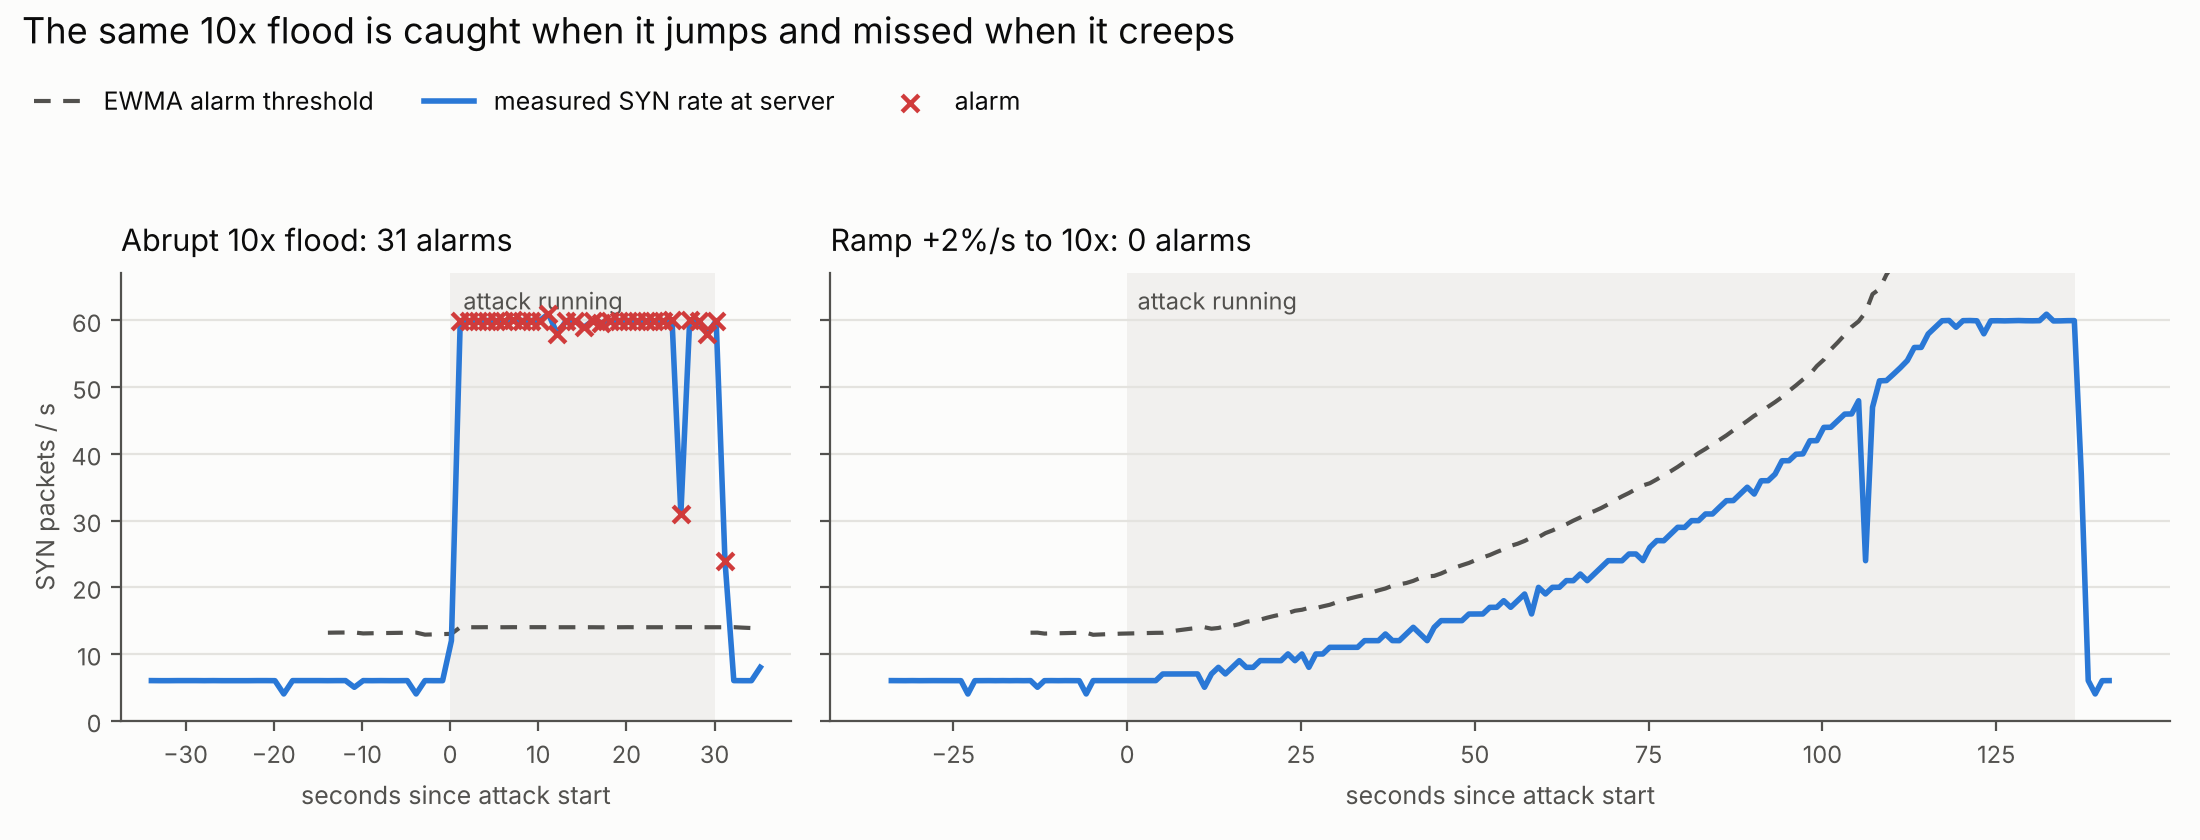
\includegraphics[width=\linewidth]{step2_ramp_vs_abrupt.png}
  \caption{The Same 10$\times$ Flood, Abrupt and as a Slow Ramp}
  \label{fig:frog}
\end{figure}

\begin{table}[H]
\centering
\caption{Frog-Boiling Attack against the EWMA Detector}
\label{tab:frog}
\begin{tabular}{lcccc}
\toprule
Attack & Measured / planned & Reached & EWMA alarms & First alarm \\
\midrule
Abrupt $10\times$ & 0.98  & $9.7\times$  & 31 & 1.2 s \\
Ramp +2\%/s       & 0.993 & $10.3\times$ & 0  & never \\
\bottomrule
\end{tabular}
\end{table}

\subsection{Lightweight Detector Results}
All five detector configurations were evaluated with five repeats each on the
abrupt flood, the slow ramp (+0.5\% per second) and a real flash crowd
(Table~\ref{tab:detection}).

\begin{table}[H]
\centering
\caption{Detection Results (5 Runs per Scenario)}
\label{tab:detection}
\small
\begin{tabular}{lccc}
\toprule
& Abrupt $10\times$ flood & Slow ramp (+0.5\%/s) & Flash crowd \\
Detector & detected (first alarm) & detected (amplification) & false alarms \\
\midrule
Static           & 5/5 (1.1 s) & 5/5 ($2.17 \pm 0.11\times$) & 5/5 \\
EWMA             & 5/5 (1.1 s) & 1/5 ($10.21\times$)          & 1/5 \\
Half-Space Trees & 5/5 (1.1 s) & 1/5                          & 5/5 \\
\textbf{EWMA + gate} & \textbf{5/5 (1.1 s)} & \textbf{5/5 ($2.89 \pm 0.11\times$)} & \textbf{1/5} \\
HST + gate       & 5/5 (1.1 s) & 5/5 ($1.93 \pm 1.02\times$) & 5/5 \\
\bottomrule
\end{tabular}
\end{table}

The results show that:
\begin{itemize}
  \item Every detector catches the abrupt flood in about one second.
  \item Without the gate, the adaptive detectors are boiled: EWMA caught the slow
  ramp in only 1 of 5 runs, and only when it was already $10.2\times$. The
  single Half-Space Trees detection was an alarm on a brief dip in traffic, not
  on the attack.
  \item Static catches the ramp, but it raises a false alarm in every flash
  crowd, at about $2.85\times$. Half-Space Trees also false-alarms on every
  crowd.
  \item \textbf{EWMA + gate is the only configuration that catches the slow
  attack in every run and stays quiet for real users.} The single crowd false
  alarm is EWMA's own: it happens in the same run with and without the gate.
  \item The gate fixes \emph{what} a detector learns, not \emph{how} it raises
  alarms, so HST + gate still false-alarms on crowds.
\end{itemize}

One run of each scenario is shown in Figure~\ref{fig:detectors}. In the ramp the
gate closed at $1.43\times$, exactly as predicted from $1/m < 0.7$. The predicted
alarm level, with the baseline frozen near $1.43\times$, was about $2.9\times$;
the measured value over five runs was $2.89 \pm 0.11\times$. In the flash crowd
the gate never closed, because real users complete their connections.

\begin{figure}[H]
  \centering
  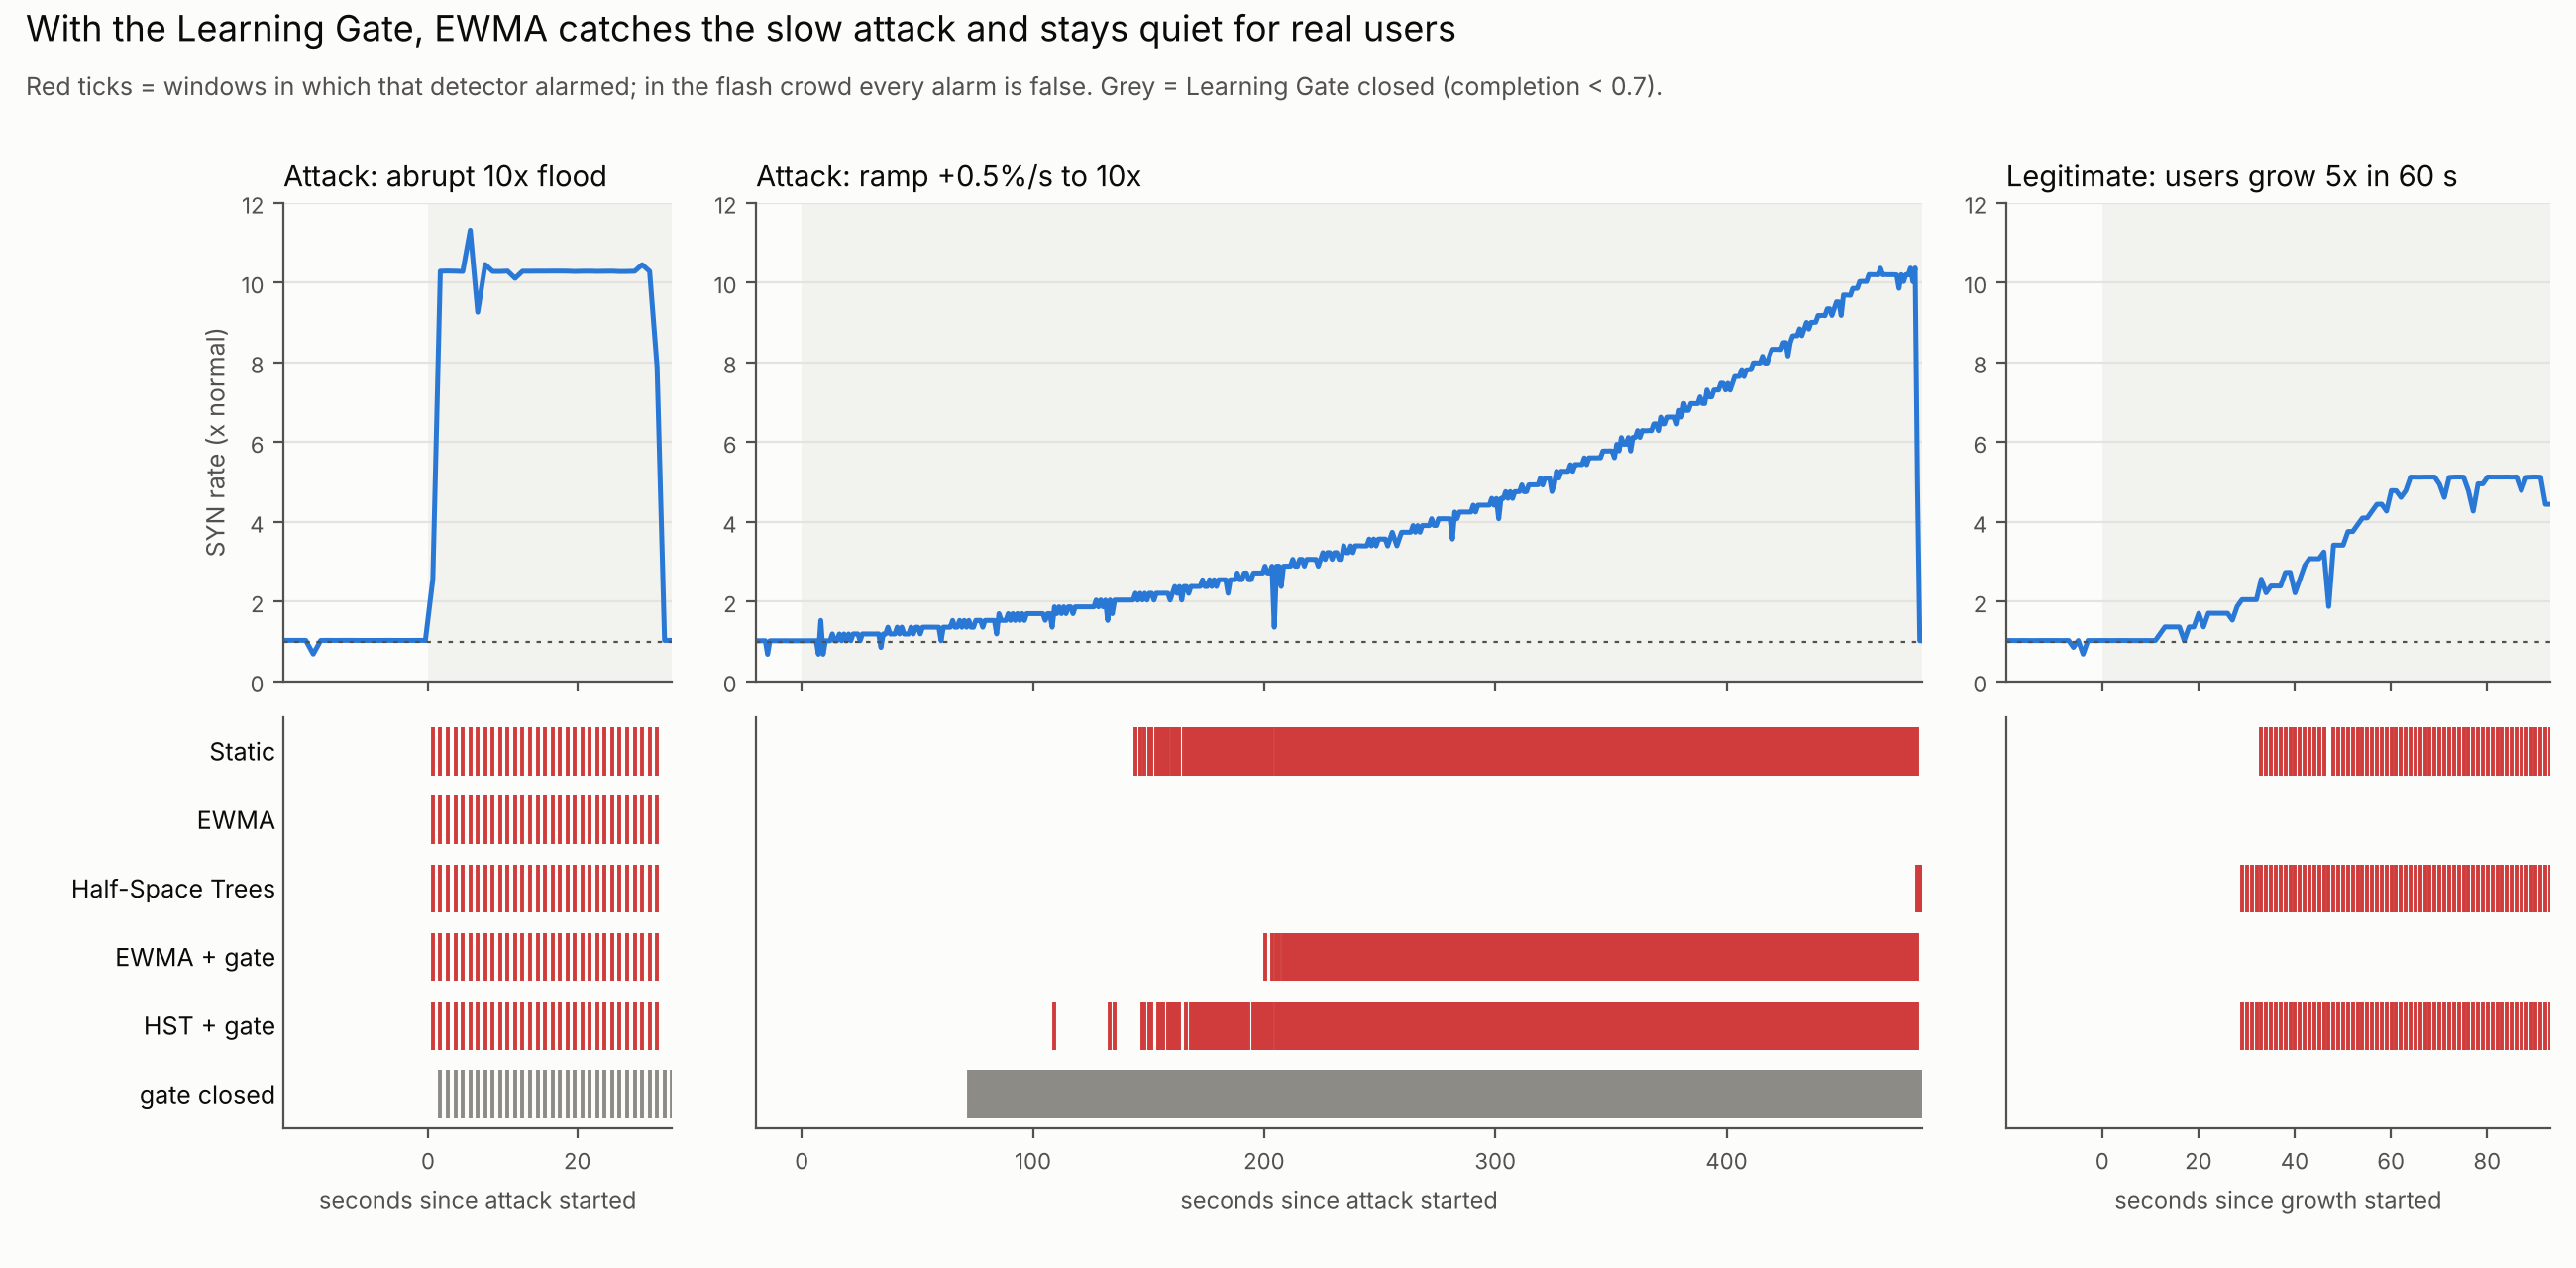
\includegraphics[width=\linewidth]{step4_detectors.png}
  \caption{Detector Alarms with and without the Learning Gate}
  \label{fig:detectors}
\end{figure}

\textbf{Choice of the threshold $\tau$.} Replaying all recorded runs with other
values of $\tau$ (Figure~\ref{fig:tau}) shows that a higher $\tau$ freezes the
baseline earlier, so the slow attack is caught at a smaller size: $5.65\times$ at
$\tau = 0.3$, $2.89\times$ at $\tau = 0.7$ and $2.34\times$ at $\tau = 0.95$. The
false alarms on real crowds did not change with $\tau$ (1 of 5 runs at every
value), because real users keep the completion ratio near 1. The value
$\tau = 0.7$ was chosen as a balance that leaves room for normal connection
failures.

\begin{figure}[H]
  \centering
  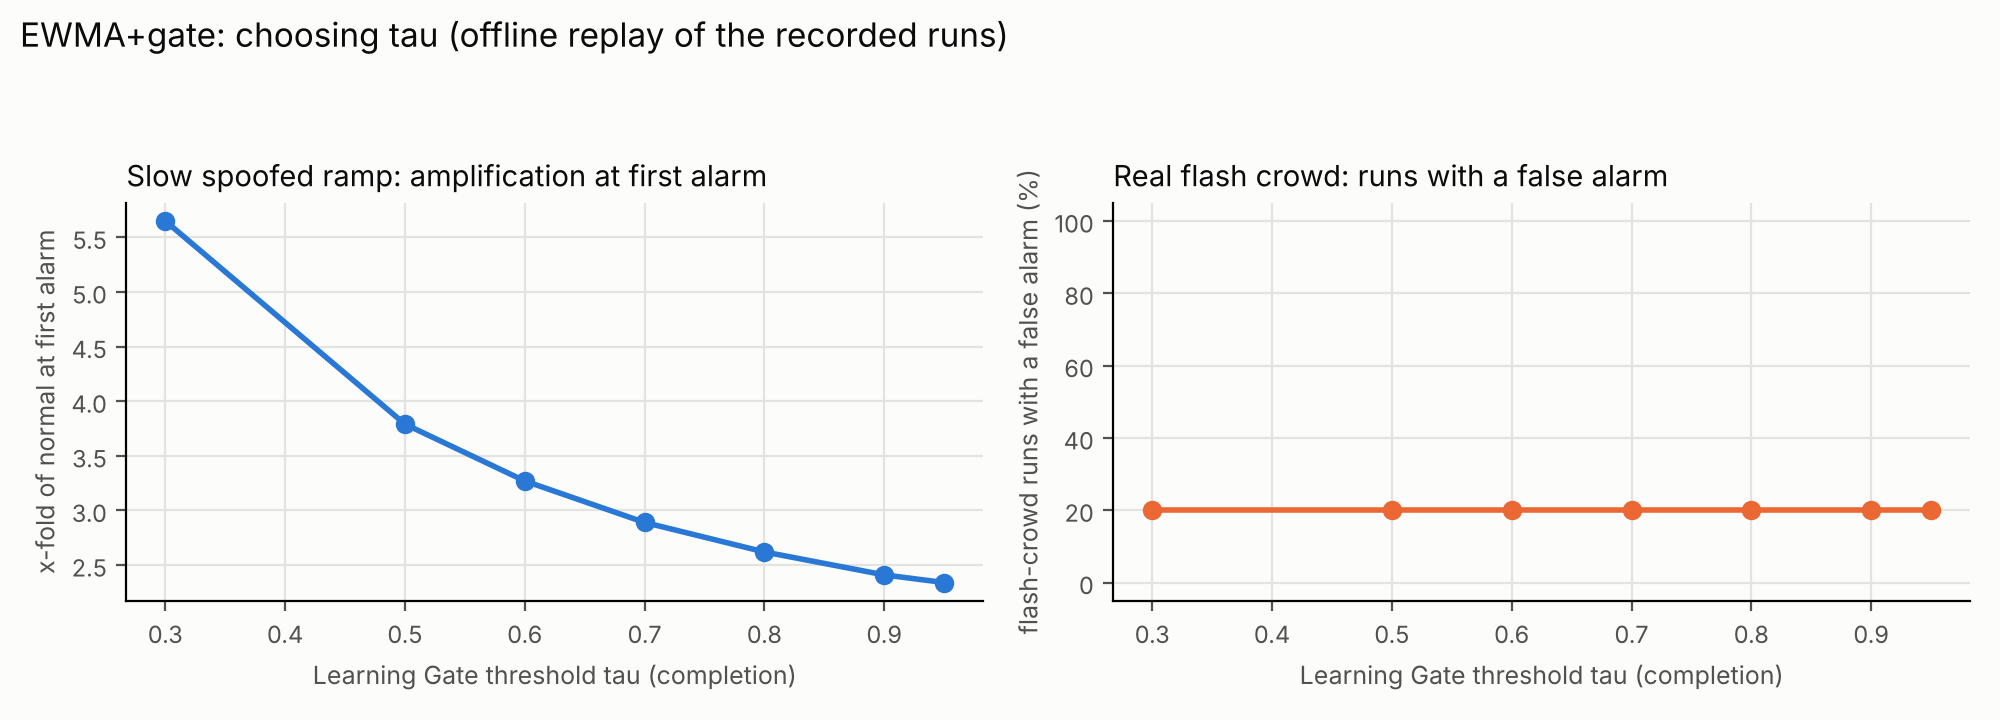
\includegraphics[width=\linewidth]{fig_tau.png}
  \caption{Effect of the Gate Threshold $\tau$ (Offline Replay)}
  \label{fig:tau}
\end{figure}

\textbf{Attack during warm-up.} The fix described in Section~8.3 was tested with
an abrupt flood that started 10 seconds after the users, inside the warm-up
(Table~\ref{tab:early}). The first version of the gate and the detectors without
a gate learned the flood as normal and never raised an alarm. With the warm-up
gated, both EWMA + gate and HST + gate caught it in all three runs, 49 seconds
after it started, once the waiting warm-up ended. Replaying all 48 earlier
gated results with the new code gives exactly the same answers, so the other
results are not affected by the fix.

\begin{table}[H]
\centering
\caption{Flood Starting 10 s after the Users (3 Runs)}
\label{tab:early}
\begin{tabular}{lc}
\toprule
Detector & Detected \\
\midrule
Static, EWMA, Half-Space Trees          & 0/3 \\
EWMA + gate, first version              & 0/3 \\
HST + gate, first version               & 0/3 \\
\textbf{EWMA + gate, warm-up gated}     & \textbf{3/3} (49 s after the start) \\
\textbf{HST + gate, warm-up gated}      & \textbf{3/3} (49 s after the start) \\
\bottomrule
\end{tabular}
\end{table}

\subsection{SYN Flood Experiment Results}
\textbf{Speed of the ramp.} The slow attack was repeated at three growth rates
(Table~\ref{tab:growth}). EWMA + gate caught it in every run at every speed, at
about $2.7$--$2.9\times$. Plain EWMA caught it in only 2 of 11 runs, and only
once the attack was already more than $10\times$ the normal rate.

\begin{table}[H]
\centering
\caption{Detection at Different Ramp Speeds (Detected, Amplification at Alarm)}
\label{tab:growth}
\small
\begin{tabular}{lccc}
\toprule
Detector & +0.5\%/s (5 runs) & +1\%/s (3 runs) & +2\%/s (3 runs) \\
\midrule
Static           & 5/5 ($2.17\times$) & 3/3 ($2.25\times$) & 3/3 ($2.19\times$) \\
EWMA             & 1/5 ($10.21\times$) & 1/3 ($15.23\times$) & 0/3 \\
Half-Space Trees & 1/5 & 2/3 ($3.27\times$) & 3/3 ($5.04\times$) \\
\textbf{EWMA + gate} & \textbf{5/5 ($2.89\times$)} & \textbf{3/3 ($2.83\times$)} & \textbf{3/3 ($2.72\times$)} \\
HST + gate       & 5/5 ($1.93\times$) & 3/3 ($1.96\times$) & 3/3 ($2.54\times$) \\
\bottomrule
\end{tabular}
\end{table}

\textbf{Distributed attack.} The attack was then split over three hosts on all
three switches (h1, h11 and h12), with nine further runs
(Table~\ref{tab:distributed}). The results match the single-attacker runs. This
is expected, since the detector watches the total traffic arriving at the
server, so the number of machines that send it does not matter.

\begin{table}[H]
\centering
\caption{Distributed Attack (3 Hosts) Compared with a Single Attacker}
\label{tab:distributed}
\small
\begin{tabular}{lcc}
\toprule
& 3 attacker hosts & 1 attacker host \\
\midrule
Abrupt $10\times$: caught by every detector & 2/2, about 1 s & 5/5, 1.1 s \\
Ramp +1\%/s: EWMA + gate & \textbf{2/2 at $3.09\times$} & 3/3 at $2.83\times$ \\
Ramp +1\%/s: plain EWMA  & 0/2 & 1/3 \\
Completing bots: EWMA + gate & 0/1 & 0/3 \\
Bypass mitigation: requests failed or delayed & 0.7\% (none: 20.6\%) & 0.4\% (none: 34.5\%) \\
\bottomrule
\end{tabular}
\end{table}

\textbf{Completing bots (limitation).} Bots that use real addresses and finish
real HTTP requests look like real users to the gate: their connections complete,
so the gate stays open and EWMA + gate missed them in all three runs. Static
and Half-Space Trees did raise alarms, but they also raise alarms on every flash
crowd. The optional drift budget catches these bots (3 of 3 runs for
$\delta \le 2\%$ per second), but it then raises a false alarm on every real
flash crowd (5 of 5), so it is a trade-off rather than a fix
(Table~\ref{tab:drift}). Such application-layer floods need application-level
defences.

\begin{table}[H]
\centering
\caption{Drift Budget $\delta$ with EWMA + Gate (Offline Replay)}
\label{tab:drift}
\begin{tabular}{lccc}
\toprule
$\delta$ per second & Slow ramp detected & Completing bots detected & Crowd false alarms \\
\midrule
off            & 5/5 & 0/3 & 1/5 \\
5\%            & 5/5 & 0/3 & 1/5 \\
2\%            & 5/5 & 3/3 & 5/5 \\
1\%            & 5/5 & 3/3 & 5/5 \\
0.5\%          & 5/5 & 3/3 & 5/5 \\
\bottomrule
\end{tabular}
\end{table}

\subsection{Selective Mitigation Results}
The mitigation was evaluated with three policies: no mitigation, a plain SYN
meter, and the meter with verified-client bypass (Table~\ref{tab:mitigation},
three runs each). In the flood and ramp scenarios the alarm came from EWMA +
gate. In the flash crowd, Static was used, to see what a \emph{false} alarm
costs real users.

\begin{table}[H]
\centering
\caption{Effect of Mitigation on Real Users and on the Server (3 Runs Each)}
\label{tab:mitigation}
\small
\begin{tabular}{llccc}
\toprule
Scenario & Policy & Requests OK & Failed/delayed & Half-open peak \\
\midrule
Abrupt $10\times$ & none              & 99.5\%  & 34.5\% & 385 \\
                  & plain meter       & 43.2\%  & 87.7\% & 257 \\
                  & \textbf{meter + bypass} & \textbf{99.7\%} & \textbf{0.4\%} & \textbf{258} \\
\midrule
Ramp +1\%/s       & none              & 99.9\%  & 2.9\%  & 385 \\
                  & plain meter       & 88.7\%  & 21.1\% & 258 \\
                  & \textbf{meter + bypass} & \textbf{100\%} & \textbf{0.0\%} & \textbf{258} \\
\midrule
Flash crowd       & none              & 100\%   & 0.0\%  & 0 \\
(Static false alarm) & plain meter    & 91.6\%  & 25.8\% & 0 \\
                  & meter + bypass    & 100\%   & 0.0\%  & 1 \\
\bottomrule
\end{tabular}
\end{table}

The results show that:
\begin{itemize}
  \item Without mitigation the server's half-open queue fills up (385
  connections, the point where Linux starts refusing new SYNs), and about a
  third of the user requests are delayed.
  \item A plain meter makes things worse for users: 87.7\% of requests failed or
  were delayed, because most of the SYNs that the meter lets through are fake.
  \item With the verified-client bypass, only 0.4\% of requests were affected,
  and the queue stayed at about 258. That level is just above half of the
  queue, where Linux starts removing old half-open entries early; the meter
  does not push it lower.
  \item When Static raised a false alarm during a flash crowd, the plain meter
  hurt a quarter of the requests, while the bypass kept every user unaffected.
\end{itemize}

Figure~\ref{fig:timeline} shows one abrupt flood second by second. The
mitigation started in the same second as the alarm (1 second after the attack
started). Without mitigation many users had to wait an extra 1--2 seconds; with
the bypass every user connected immediately.

\begin{figure}[H]
  \centering
  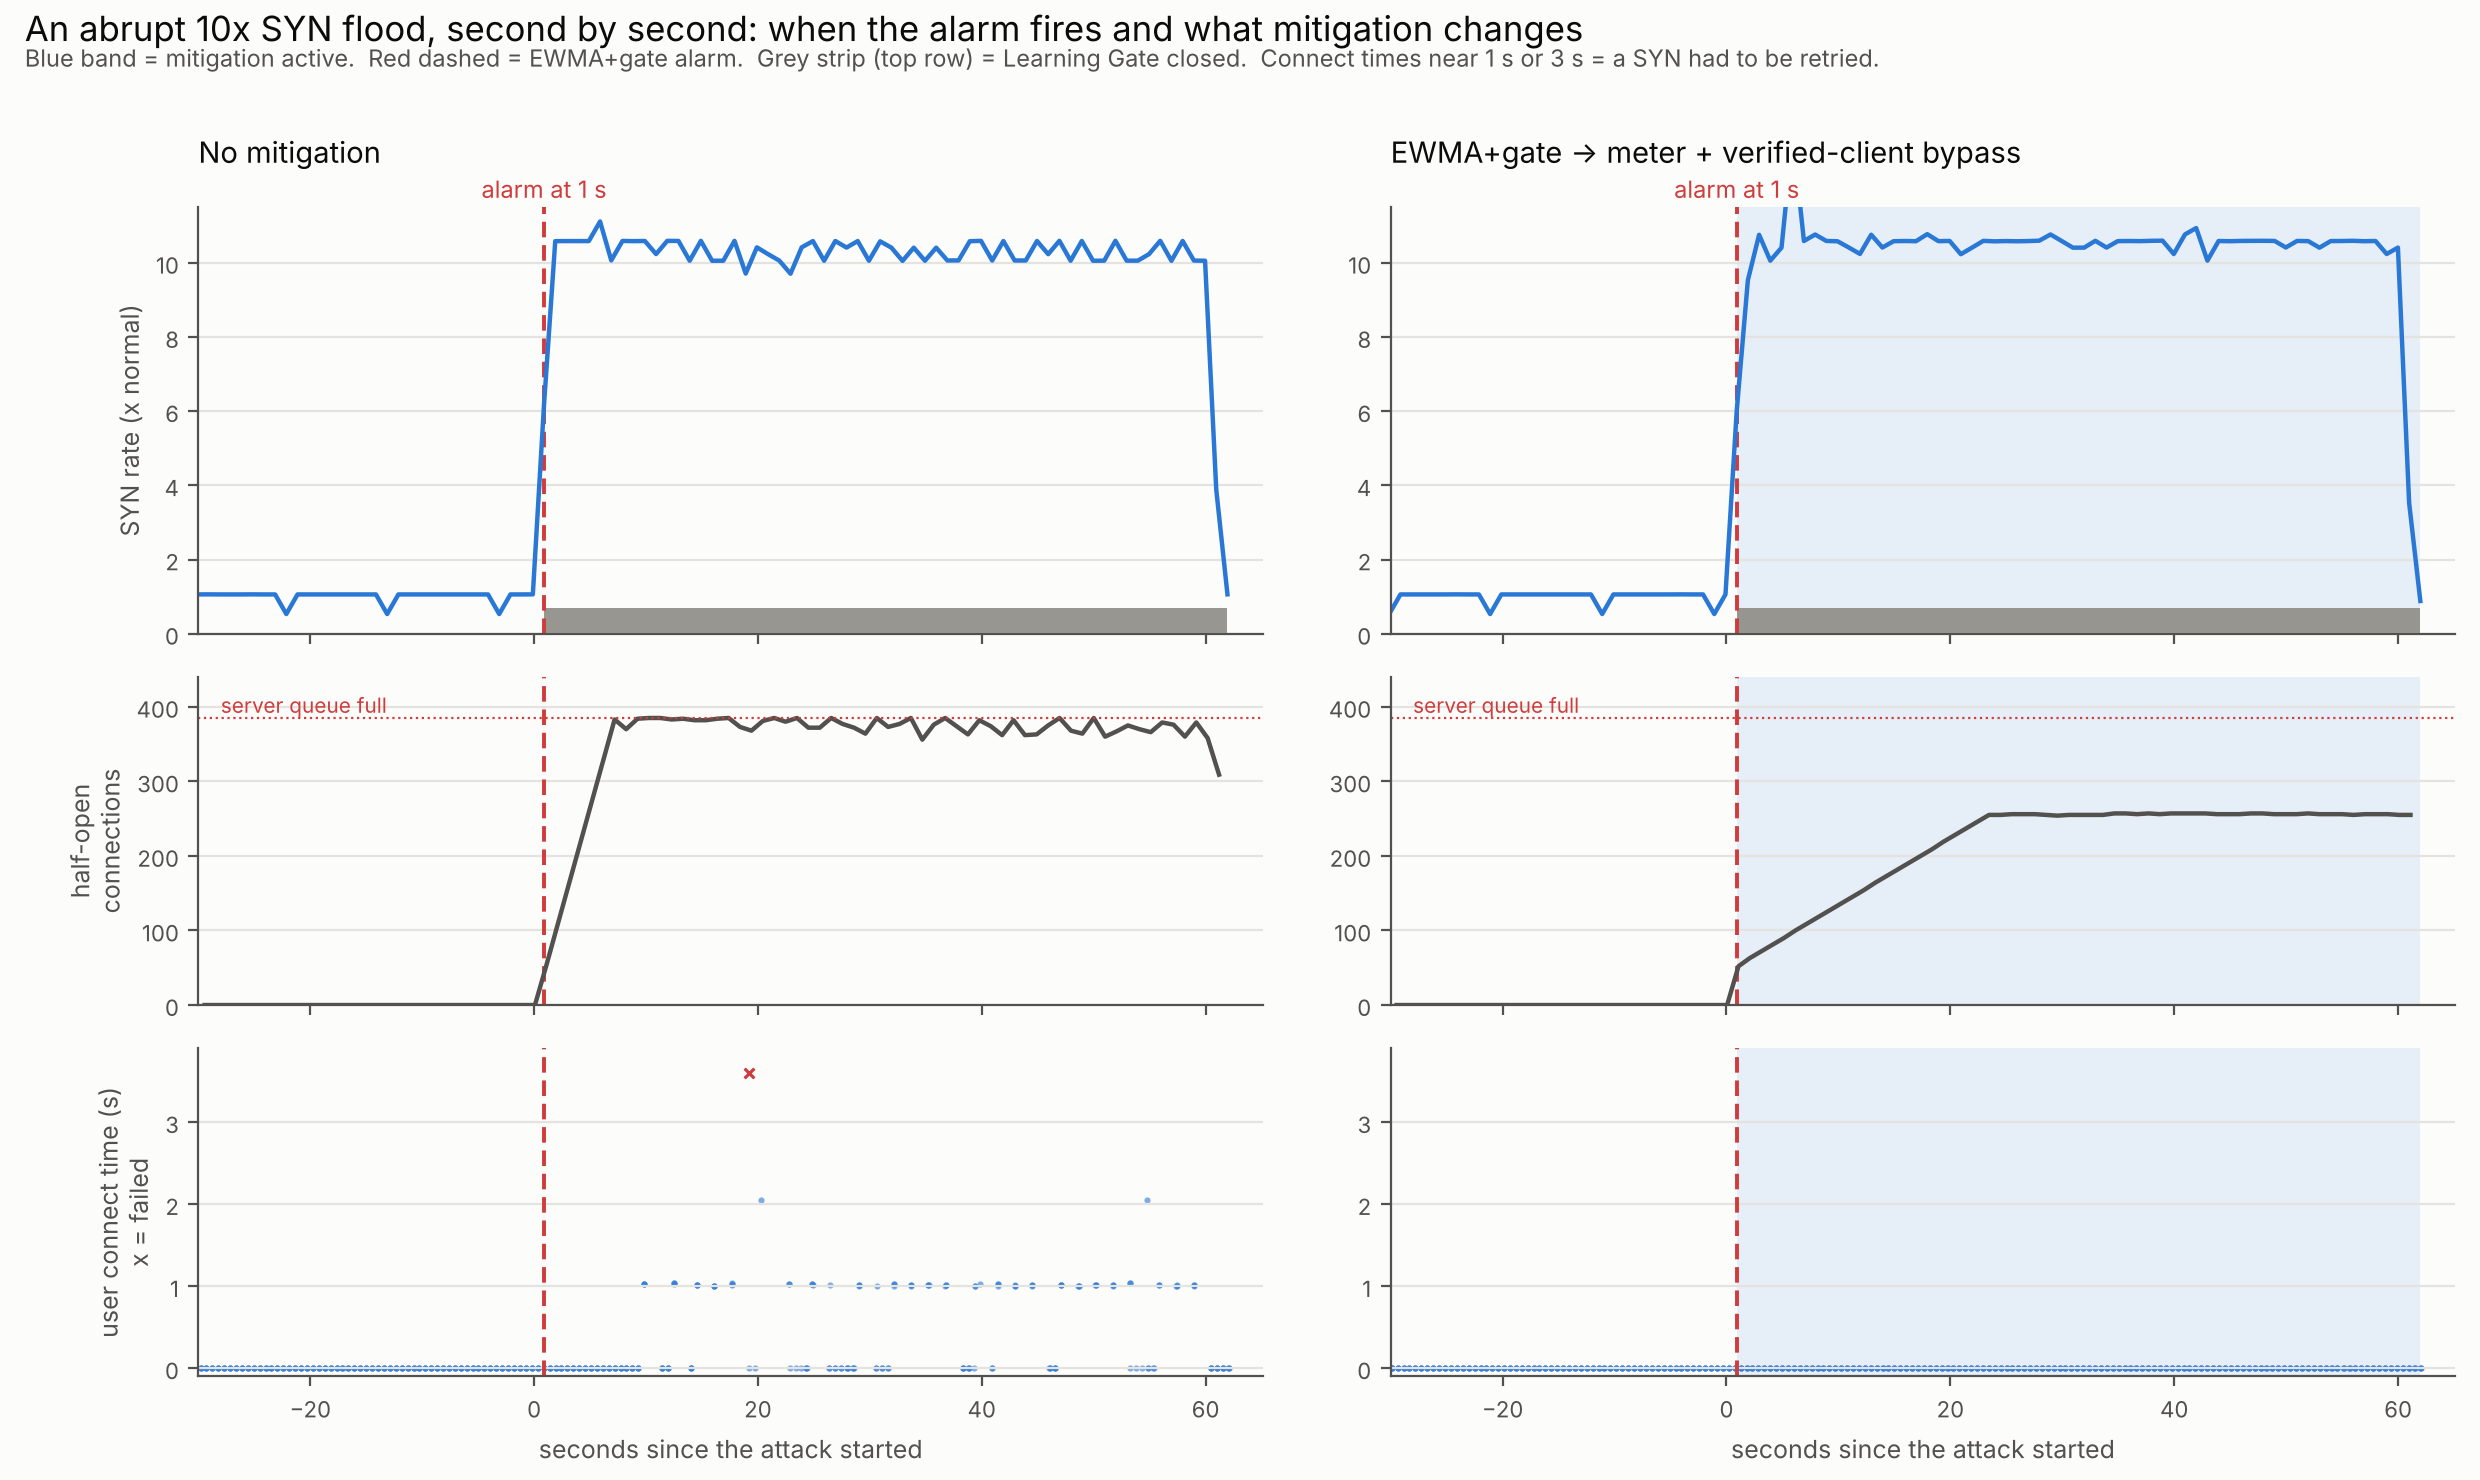
\includegraphics[width=\linewidth]{fig_timeline_abrupt.png}
  \caption{Abrupt Flood with and without Mitigation, Second by Second}
  \label{fig:timeline}
\end{figure}

\begin{figure}[H]
  \centering
  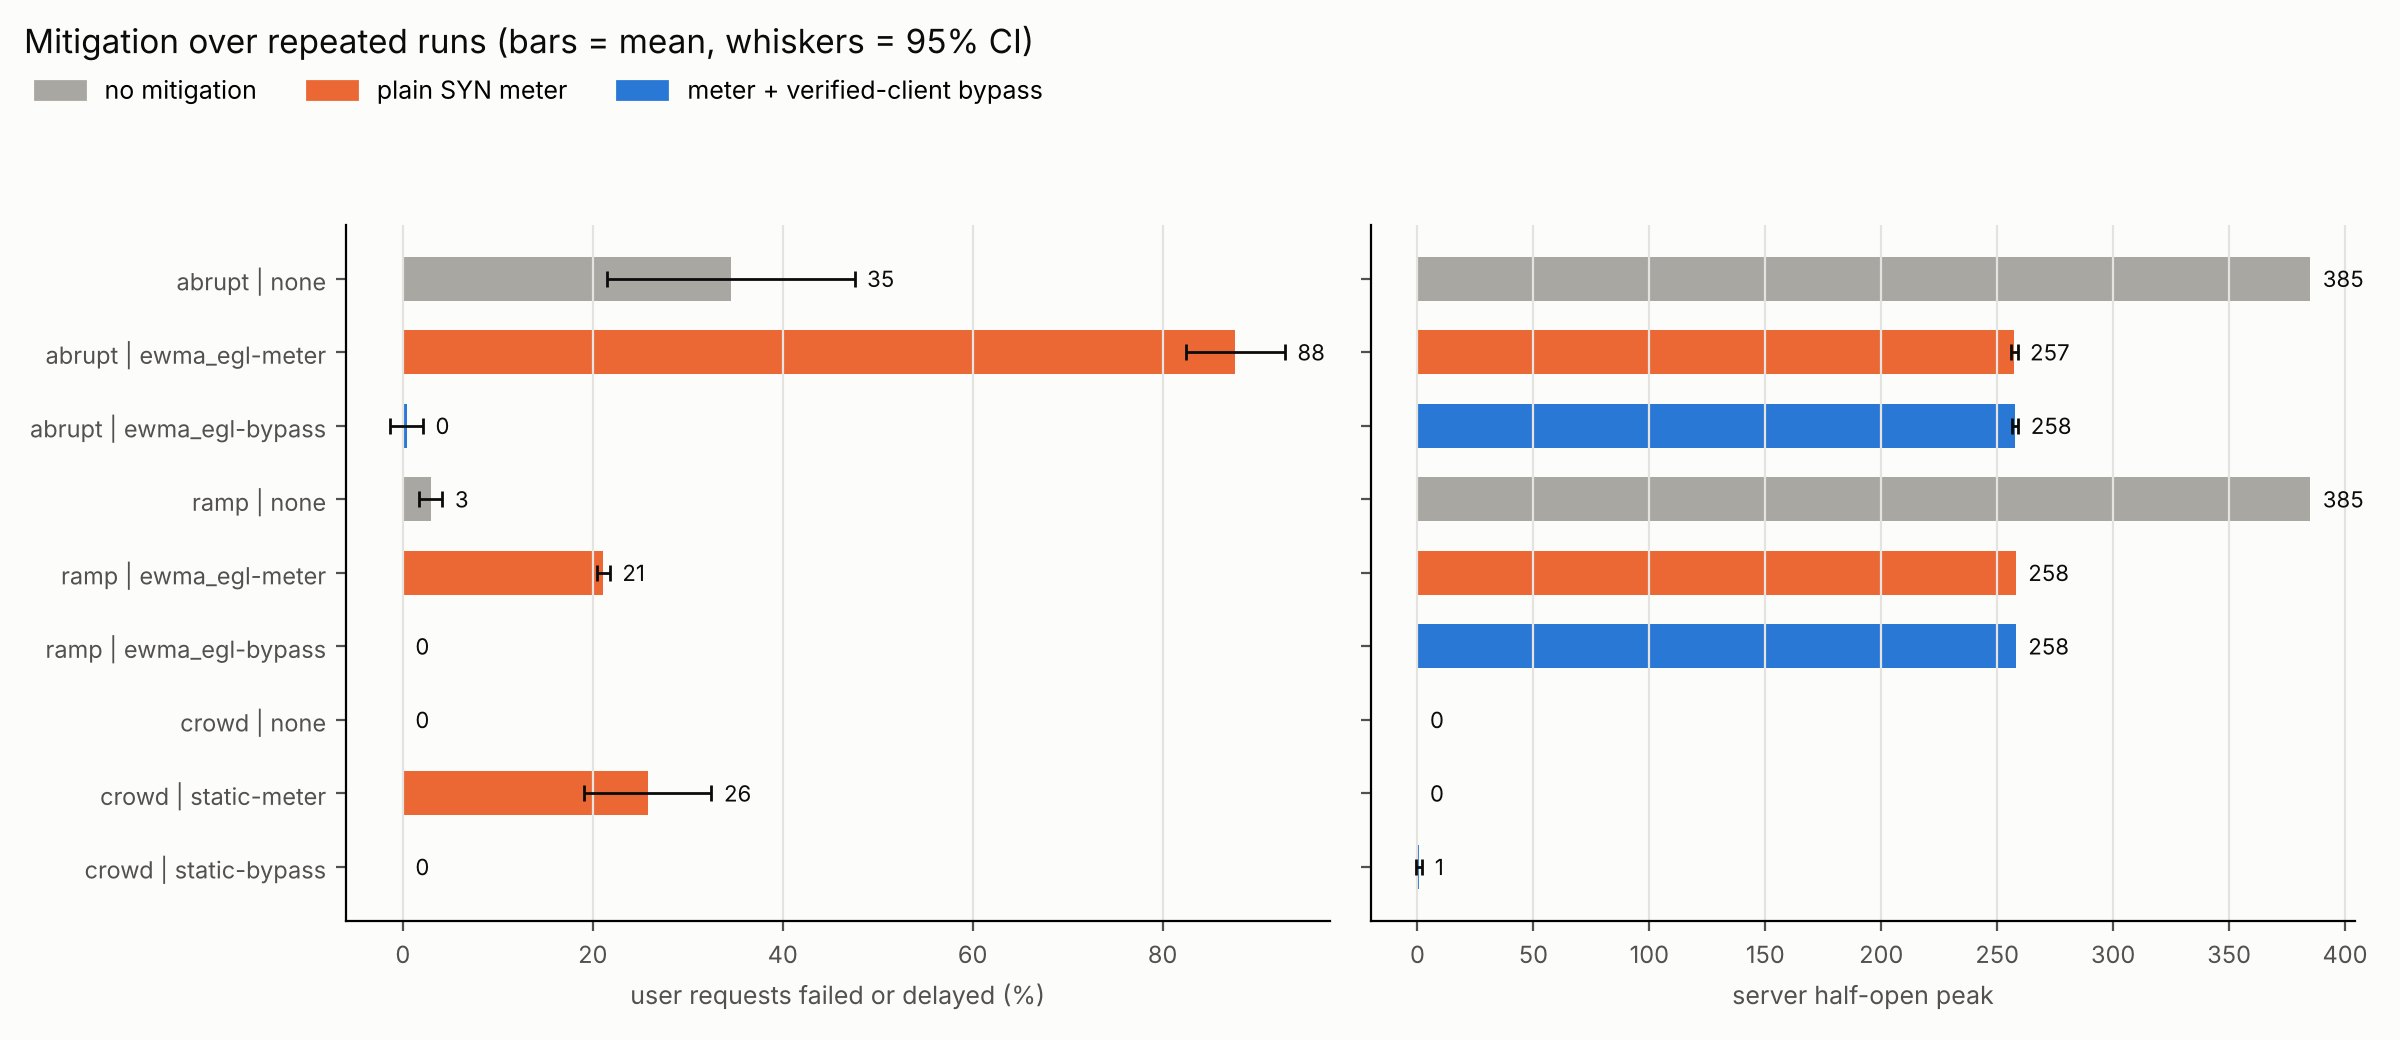
\includegraphics[width=\linewidth]{fig_mitigation.png}
  \caption{Requests Failed or Delayed under Each Mitigation Policy}
  \label{fig:mitigation}
\end{figure}

The meter limit was also varied on the abrupt flood (Table~\ref{tab:margin}).
With the bypass in place, all three limits kept the affected requests between
1\% and 1.5\%, so the result does not depend strongly on this setting.

\begin{table}[H]
\centering
\caption{Meter Limit with Verified-Client Bypass (Abrupt Flood, 2 Runs Each)}
\label{tab:margin}
\begin{tabular}{lccc}
\toprule
Meter limit & Requests OK & Failed or delayed & Half-open peak \\
\midrule
$0.5\times$ trusted baseline & 98.8\% & 1.4\% & 256 \\
$1.0\times$ trusted baseline & 98.8\% & 1.1\% & 256 \\
$2.5\times$ trusted baseline & 99.1\% & 1.2\% & 259 \\
\bottomrule
\end{tabular}
\end{table}

\subsection{Findings from Literature Survey}
The following conclusions were drawn from a systematic review of the literature
and the implemented system:
\begin{itemize}
  \item DDoS mitigation in SDN still remains an open problem, with no general
  solution due to the similarity between attack traffic and legitimate flash
  crowd traffic. This is a challenge known as the flash crowd disambiguation
  problem.
  \item The SDN controller is a single point of failure, both computationally
  through Packet-In flood exhaustion and topologically through southbound
  channel saturation. Effective mitigation should address both.
  \item Entropy-based detection methods perform reliably against volume-based
  packet flooding attacks but may fail against Low-Rate DDoS attacks. Therefore,
  a secondary ML-based model is required for detecting stealthier attacks.
  \item P4 programmable switches allow computation and detection of obvious
  attack traffic at the data plane, reducing the detection logic executed by the
  controller.
  \item Multi-Agent Systems are suitable for distributed SDN setups with multiple
  controllers and can help controllers share threat information more
  efficiently.
  \item \textbf{From the implemented system:} detectors that keep learning,
  including the online ML detector (Half-Space Trees), can be slowly poisoned.
  A $10\times$ flood went completely unnoticed when it was raised slowly.
  \item Traffic volume alone cannot separate a slow attack from a growing crowd
  of real users. Evidence of completed connections can: gating what the detector
  learns on this evidence caught every slow attack while real crowds were still
  accepted.
  \item Mitigation must protect real users, not only the server. A plain rate
  limit hurt more users than the flood itself, while a bypass for verified
  clients kept almost every request unaffected.
  \item The remaining limitations are: bots that complete real connections pass
  the gate; the gate does not change how a detector raises alarms; brand-new
  visitors who arrive during an attack must first pass the meter; the evidence
  is specific to TCP; and the testbed is small, with a single controller.
\end{itemize}

% =====================================================================
\newpage
\section*{References and Datasets}
% =====================================================================
\renewcommand{\refname}{References}
\begin{thebibliography}{9}
\bibitem{sinha2025} Mitali Sinha, \emph{A Comprehensive Survey of DDoS Attack
Defense Systems for Different SDN Architectures}, Computer Networks, 2025.
\bibitem{wang_survey} Wei Wang, Yong Liu, Qian Meng, and Zihang Chen, \emph{DDoS
Attack Detection and Defense Techniques in Software Defined Networks: A Survey},
Computer Networks.
\bibitem{antidote} Benjamin I.\ P.\ Rubinstein, Blaine Nelson, Ling Huang,
Anthony D.\ Joseph, Shing-hon Lau, Satish Rao, Nina Taft, and J.\ D.\ Tygar,
\emph{ANTIDOTE: Understanding and Defending against Poisoning of Anomaly
Detectors}, ACM Internet Measurement Conference (IMC), 2009.
\bibitem{chantin} Eric Chan-Tin, Daniel Feldman, Nicholas Hopper, and Yongdae
Kim, \emph{The Frog-Boiling Attack: Limitations of Anomaly Detection for Secure
Network Coordinate Systems}, SecureComm, 2009.
\bibitem{zhang2026} Zhaoyang Zhang, Shen Wang, Ahmad Taha, Elias Bou-Harb, and
Xiaofeng Tao, \emph{When Time Meets Space: Entropy Integration and Dynamic
Threshold for Adaptive DDoS Detection in SDN}, arXiv:2608.15642, 2026.
\bibitem{tan2011} Swee Chuan Tan, Kai Ming Ting, and Tony Fei Liu, \emph{Fast
Anomaly Detection for Streaming Data}, International Joint Conference on
Artificial Intelligence (IJCAI), 2011.
\bibitem{wang2002} Haining Wang, Danlu Zhang, and Kang G.\ Shin,
\emph{Detecting SYN Flooding Attacks}, IEEE INFOCOM, 2002.
\end{thebibliography}

\subsection*{Datasets}
\begin{itemize}
  \item \textbf{SDN-based DDoS Traffic Dataset}\\
  Generated using the Mininet emulator with a Ryu controller for traffic
  classification using machine learning and deep learning techniques. The
  dataset contains 23 flow-based and port-based features collected from benign
  and malicious traffic scenarios including TCP SYN flood, UDP flood, and ICMP
  attacks. The dataset consists of 104,345 records collected over a simulation
  duration of 250 minutes.
  \item \textbf{Project measurements}\\
  All telemetry, detector verdicts, mitigation actions and user request logs of
  the 69 runs reported in Section~9 are stored as CSV and JSON files in the
  project repository, together with the scripts that produce every table and
  figure.
\end{itemize}

\end{document}
